% Created 2014-04-14 Mon 18:10
\documentclass[runningheads,a4paper]{llncs}
\usepackage[utf8]{inputenc}
\usepackage[T1]{fontenc}
\usepackage[protrusion=true,expansion=true]{microtype}
\usepackage{fixltx2e}
\usepackage{graphicx}
\usepackage{float}
\usepackage{wrapfig}
\usepackage{amsmath}
\usepackage{textcomp}
\usepackage{wrapfig}
\usepackage{marvosym}
\usepackage{wasysym}
\usepackage{amssymb}
\usepackage{hyperref}
\usepackage{microtype}
\usepackage{acronym}
\tolerance=1000
\usepackage[usenames,dvipsnames]{xcolor}
\usepackage{listings}

\urldef{\mailsa}\path|{joel.kuiper, m.a.swertz}@rug.nl|
\urldef{\mailsb}\path|iain.marshall@kcl.ac.uk|
\urldef{\mailsc}\path|byron_wallace@brown.edu|

\acrodef{ebm}[EBM]{Evidence-based Medicine}

\institute{
  University of Groningen P.O. Box 30001, 9700 RB Groningen \\ \mailsa
  \and King's College London, London SE1 3QD, UK \\ \mailsb
  \and Brown University, Providence, RI 02906, USA \\ \mailsc}

\begin{document}
\setcounter{tocdepth}{3}
\newcommand{\highlight}[1]{\colorbox{yellow}{#1}}

% Autogenerated, do not edit
\newcommand{\revisiondate}{2014-04-24}
<<<<<<< HEAD
\newcommand{\revision}{3f2c73a}
=======
\newcommand{\revision}{d58899a}
>>>>>>> 1b257ee... updates

\author{Kuiper, J\inst{1}. \and Marshall, I.J.\inst{2} \and Wallace, B.C.\inst{3} \and Swertz, M.A.\inst{1}}
\date{\texttt{revision: \revision, date: \revisiondate}}
\title{Spá: a web-based viewer for text mining in Evidence Based Medicine}


\maketitle
\begin{abstract}
Unstructured PDF documents remain the main vehicle for dissemination of scientific findings.
Those interested in gathering and assimilating data must therefore manually peruse published articles and extract from these the elements of interest.
\acl{ebm} provides a compelling illustration of this: many person-hours are spent each year extracting summary information from articles that describe clinical trials.
This represents an enormous burden, especially in light of the expotentially increasing volume of published biomedical articles.
Machine learning provides a potential means of mitigating this burden by automating extraction.
But for automated approaches to be useful to end-users, we need tools that allow domain experts to interact with, and benefit from, model predictions.
To this end, we present a web-based tool called Spá\footnote{Source code available under GPLv3 at \url{https://github.com/joelkuiper/spa} \cite{kuiper2014}; demo available at \url{http://clinici.co/}} that accepts as input an article and provides as output an automatically visually annotated rendering of this article.
More generally, Spá provides a framework for visualizing predicted full-text PDF annotations, both at the document and sentence level.
\end{abstract}

\acresetall

\section{Introduction}
\label{section:intro}

%Finding sentences or words with particular characteristics within a document is an important task in natural language processing and machine learning.
Imposing structure on full-text documents (e.g., identifying specific sentences of interest) is an important, challenging and practical task in natural language processing and machine learning.
Consider \emph{systematic reviews} -- fundamental tools in \ac{ebm} \cite{sackett1996} -- which aim to address specific clinical questions by identifying and synthesizing data from all relevant published articles.
When doing this one often needs, for example, to assess the \emph{risk of bias} for a particular study across different domains, such as bias due to improper blinding of participants and personnel.
For this task, one wants to make a summary judgement (e.g., low risk of bias) and simultaneously extract the sentences supporting that judgement.

Extracting such information from the unstructured text of clinical trial articles is a laborious process.
Machine learning methods provide the machinery to automate such extractions; as they can effectively impose the desired structure onto PDFs.
For example, we can train a classifier to automatically assess the risk of bias across different domains and simulteanously identify the sentences supporting these assessments.
We may also train a model that extracts the sample size from a paper describing a clinical trial. 
But if such technologies are to be practically useful, we need tools that visualize these model predictions and annotations.
Here we describe Spá, which aspires to realize this aim.
Spá is an open-source, web-based tool that can incorporate state-of-the-art machine learning predictors to automatically annotate PDF articles.
As a practical (and useful) demonstration of this technology, we have built a machine learning system that automatically annotates PDFs to facilitate \ac{ebm}. 
Specifically, this system leverages a multi-task model that simulteanously assesses the risk of biases across several domains, and extracts sample sizes from articles.
%Moreover, we have created machine learning systems on describing clinical trials with risk of bias predictions and extracted sample sizes.
This tool is unique in that it leverages state-of-the-art ML models applied to full-text articles to assist practitioners of \ac{ebm} (and other biomedical researchers). 
 
\begin{figure}[htb]
	\vspace{-2em}
\centering
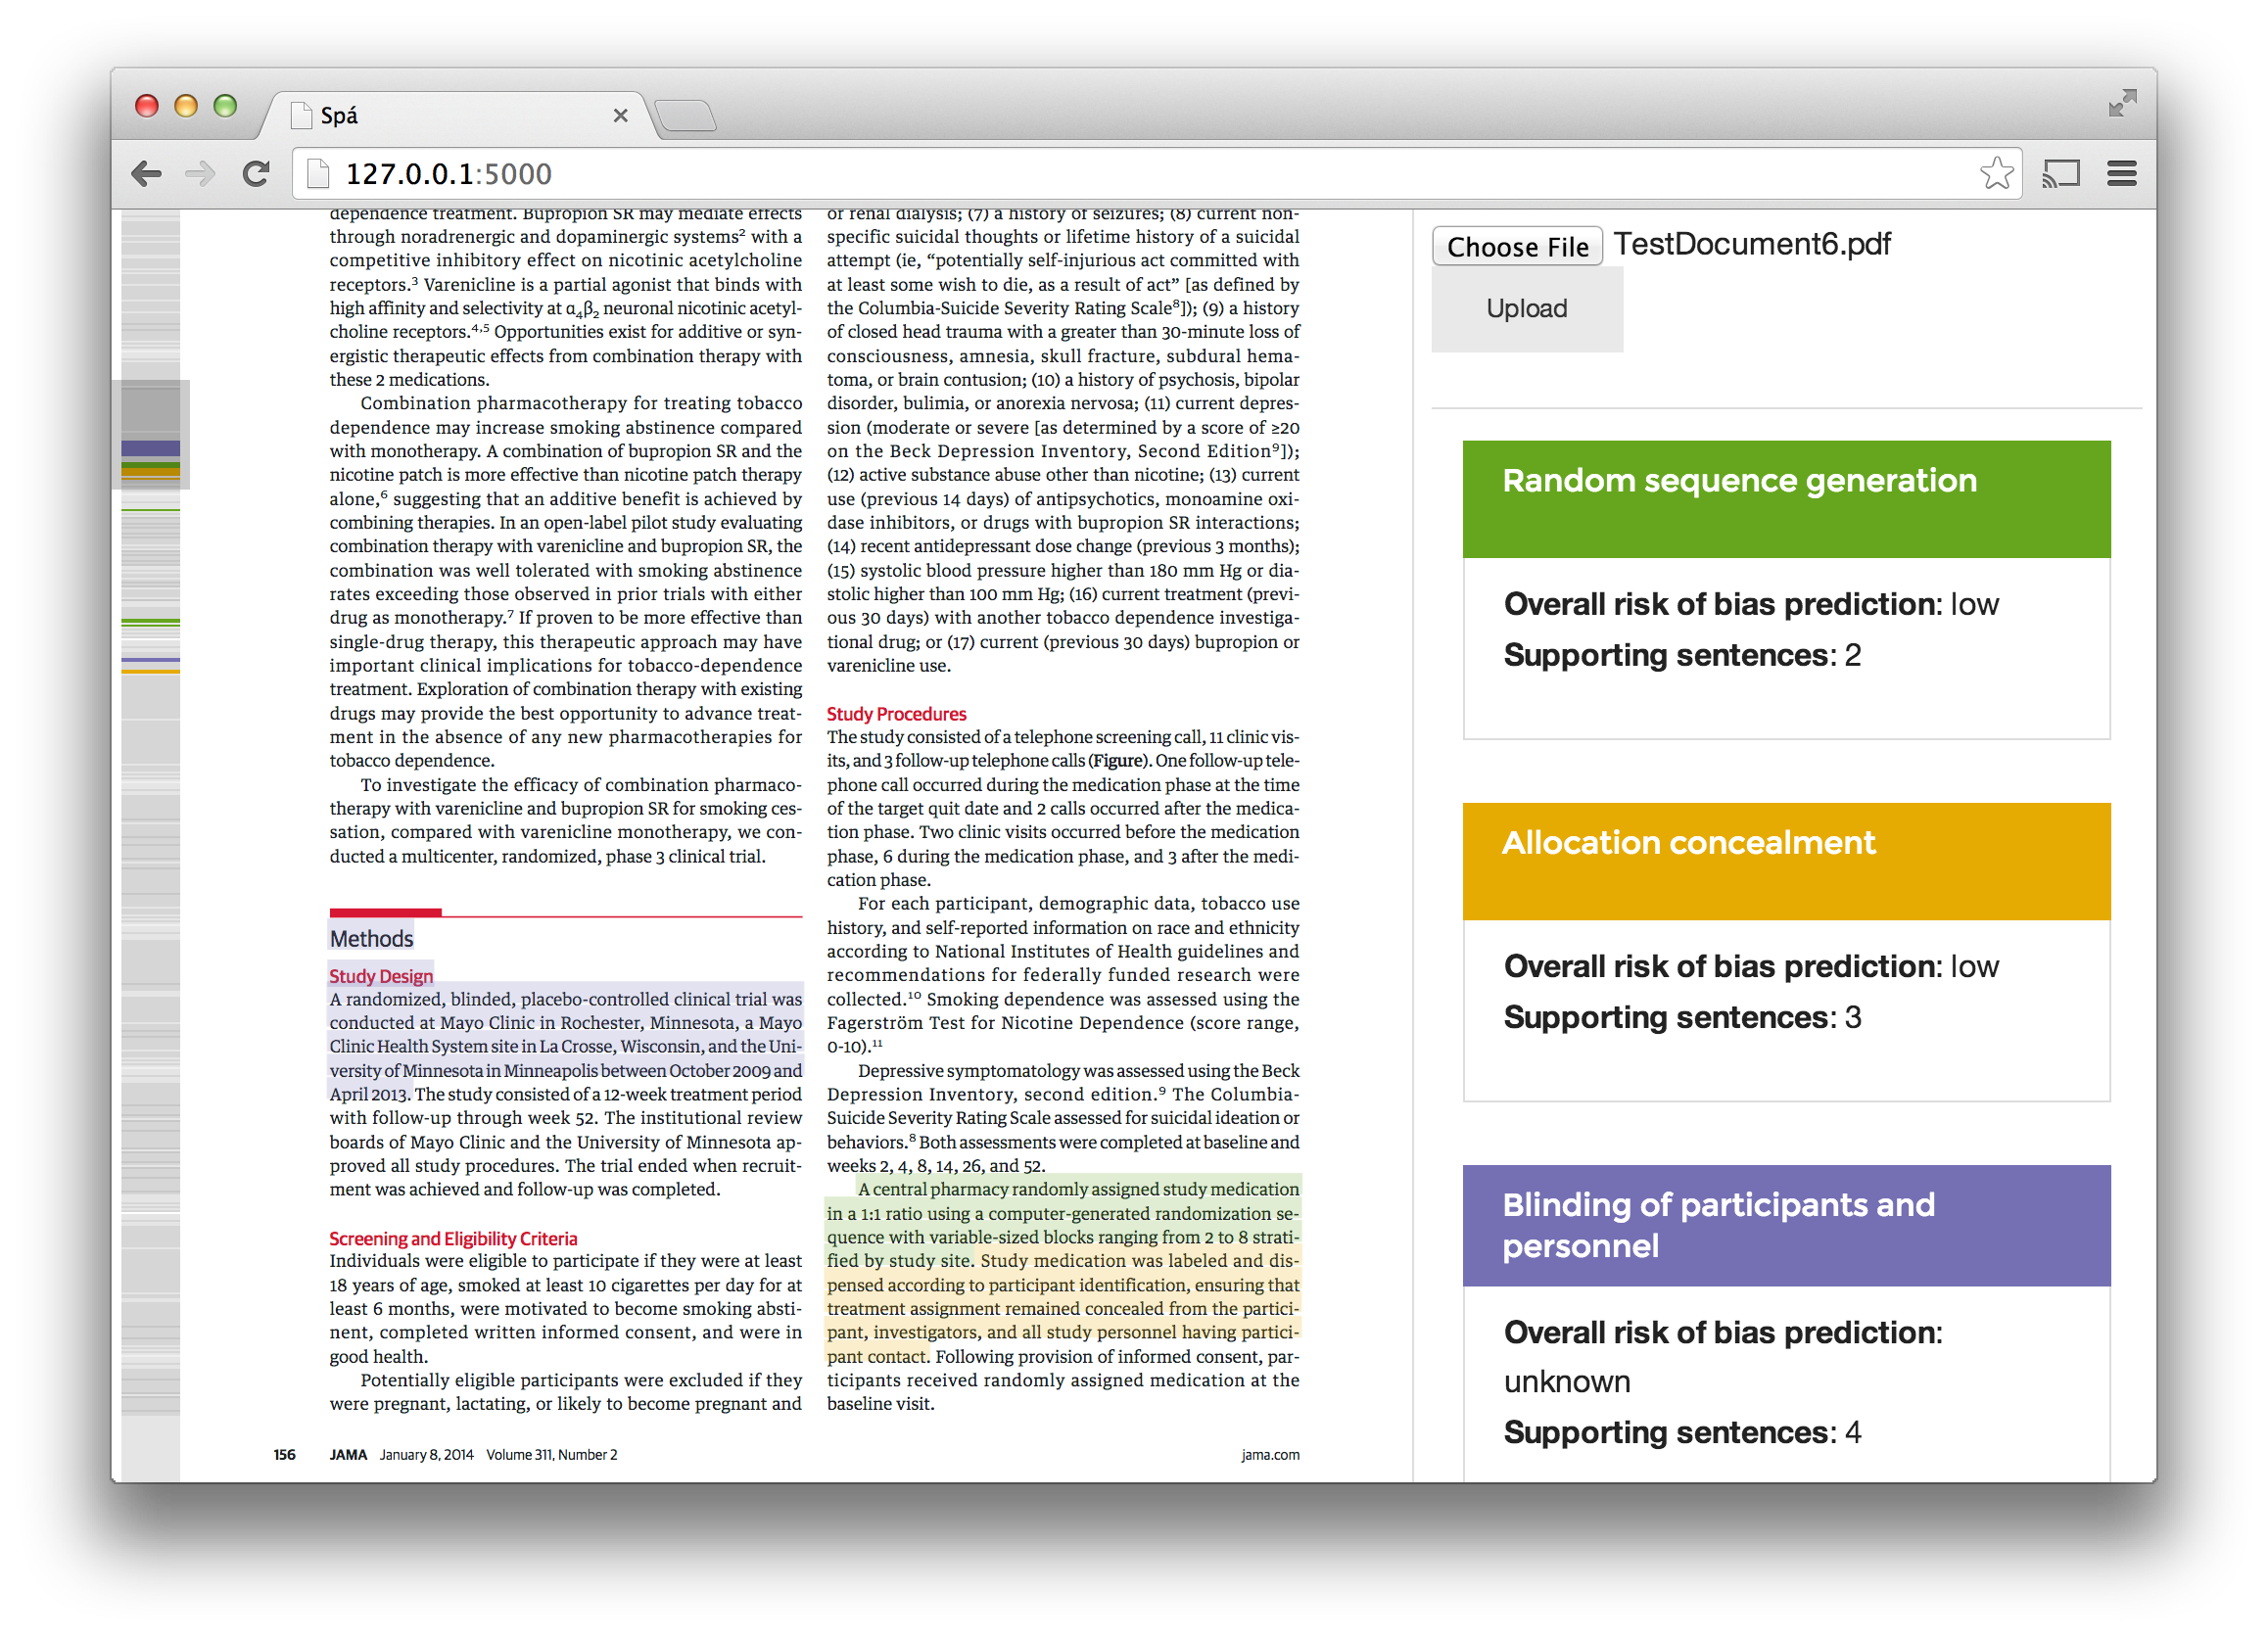
\includegraphics[width=.8\linewidth]{./images/screenshot2.png}
\vspace{-1em}
\caption{\label{fig:screenshot}Screenshot of a PDF with highlighted risk of bias. Here the risk of bias is assess to be low, for example, and one of the supporting sentences for this assessment describes the randomization procedure (highlighted in green).}
\vspace{-2em}
\end{figure}

While our application of interest is \ac{ebm}, we emphasize that the visualization tool can be used for any domain in which one wants to annotate PDFs. 
Thus the contribution of this work is two-fold, as we present:
(1) a practical tool (Spá) that incorporates cutting edge machine learning to help researchers rapidly assess the risk of biases (and sample sizes) in published biomedical articles, and,
(2) a general open-source web tool for visualizing the predictions of trained models from full-text articles.
These contributions are described further in sections \ref{section:EBM-ML} and \ref{section:architecture}, respectively.


\section{Automating \acl{ebm}}
\label{section:EBM-ML}

\subsection{Systematic Reviews}
%%% sort of redundant with above; may want to re-factor
The process of pooling and summarizing clinical trials is called \emph{systematic reviewing}, and forms the corner-stone of current \ac{ebm}.
Systematic reviewing consists of specifying a precise clinical question and accompanying study inclusion criteria, and then exhaustively searching the literature to identify eligible studies. 
Identified eligible studies are subsequently analyzed (i.e., synthesized), resulting in a summary of all of the published evidence that pertains to the clinical question of interest.
Systematic reviews thus represent a rigorous, data-driven approach to answering clinical questions. 
But conducting systematic reviews is complicated by the massive number of trials that are conducted: for example, the Cochrane Library alone indexes 286,418 trials that were conducted in the last decade \cite{valkenhoef2012}.
While methods and publishing standards are improving, many legacy publications will remain available only as PDF documents. 

Extracting information of interest from these PDFs is imperative but laborious. 
To mitigate this burden, we have constructed machine learning models that automatically extract some characteristics of interest.
Specifically, our model predicts {\it risk of biases} across different domains as a function of the texts comprising articles. 
It simultaneously extracts sentences supporting these predictions. 
We briefly outline our approach to achieving this below. 
We also note that we have a a separate model that extracts the study sample size from articles. 
Spá -- our visualization tool -- provides a framework to upload PDFs and then render these predicted annotations. 
We foresee adding additional predictors to this tool that, for example, may identify different treatment mentions within the text (e.g., drugs). 

% made a web-based tool that allows the visualization of annotations within a PDF documents, and meta-information alongside it.

\subsection{Machine Learning Approaches}

We briefly describe our model for assessing the study risk of bias (and supporting sentences) across the following domains: random sequence generation, allocation concealment, blinding of participants and personnel, blinding of outcome assessment, incomplete outcome data and selective reporting. 
To train our model, we have leveraged the Cochrane Database of Systematic Reviews (CDSR) in lieu of manually annotated data, which would be expensive to collect. 
The CDSR contains descriptions and data about clinical trials reported in existing systematic reviews. 
Briefly, we match (the full-texts of) studies to entries in the CDSR, which contains risk of bias assessments; this provides document level labels. 
The CDSR also contains sentences that annotators indicated as supporting their assessments. 
We match these strings to substrings in the PDFs to provide sentence-level supervision. 
This can thus be viewed as a \emph{distantly supervised} \cite{mintz-09,nguyen-11} approach.

 
%%%
% note that this is a little misleading right now -- we don't technically have this multi-task joint extraction thing going yet!!!
%%%
Concerning the risk of bias predictions, we have two tasks for a given article: (1) predict the overall risk of bias for each of the domains of interest, and, (2) extract the sentences that support these assessments. 
In both cases we leverage standard bag-of-words text encoding and linear-kernel support vector machines (SVMs). 
Because the risk of bias predictions are correlated (across domains), we take a \emph{multi-task} \cite{evgeniou2004} approach to classification and jointly learn a model for the domains. 
We accomplish this by way of a feature space construction that includes both shared and domain-specific terms (similar to the domain adaptation approach in \cite{daume2007}). 

With respect to the second task of sentence extraction, we \emph{jointly} assess the risk of bias associated with a given article \emph{and} the sentence(s) that support this judgement. 
Specifically, we first make sentence level predictions (using one set of trained models), and then insert features representing the tokens (words) in the predicted sentences for exploitation by the document level classifier.
Due to space constraints here, we omit further specifics of our approach, but we provide further details elsewhere \cite{marshall2014}. 
Figure \ref{fig:screenshot} shows example system output: the overall risk of bias with respect to random sequence generation is judged to be low, and supporting sentence
%More specifically, the database we leverage contains structured and semi-structured data for each systematic review. Internally, the Cochrane Collaboration stores working versions of their reviews as XML. Each review contains a wealth of (structured) data about the clinical trials that met the review inclusion criteria. There are usually multiple clinical trials described in a single review. Cochrane reviews use basic clinical trial identifiers which are unique per review (based on the first author surname and year of publication) throughout these files. It is therefore possible to extract structured data, and filtered snippets of full text data which describe a single clinical trial. Using these identifiers, we were able to obtain full structured citation data for the primary reference of all included studies across the CDSR.


% \begin{itemize}
% \item Basically show that we're using state of the art
% \item Briefly talk about cochrane DB / distant supervision
% \item KDD stuff (briefly)
% \item Multi-task stuff!
% \end{itemize}

%\vspace{-2em}
\section{Spá Architecture Overview}
\label{section:architecture}
 \vspace{-1em}
\begin{wrapfigure}{l}{0.5\textwidth}
%\centering
\begin{center}
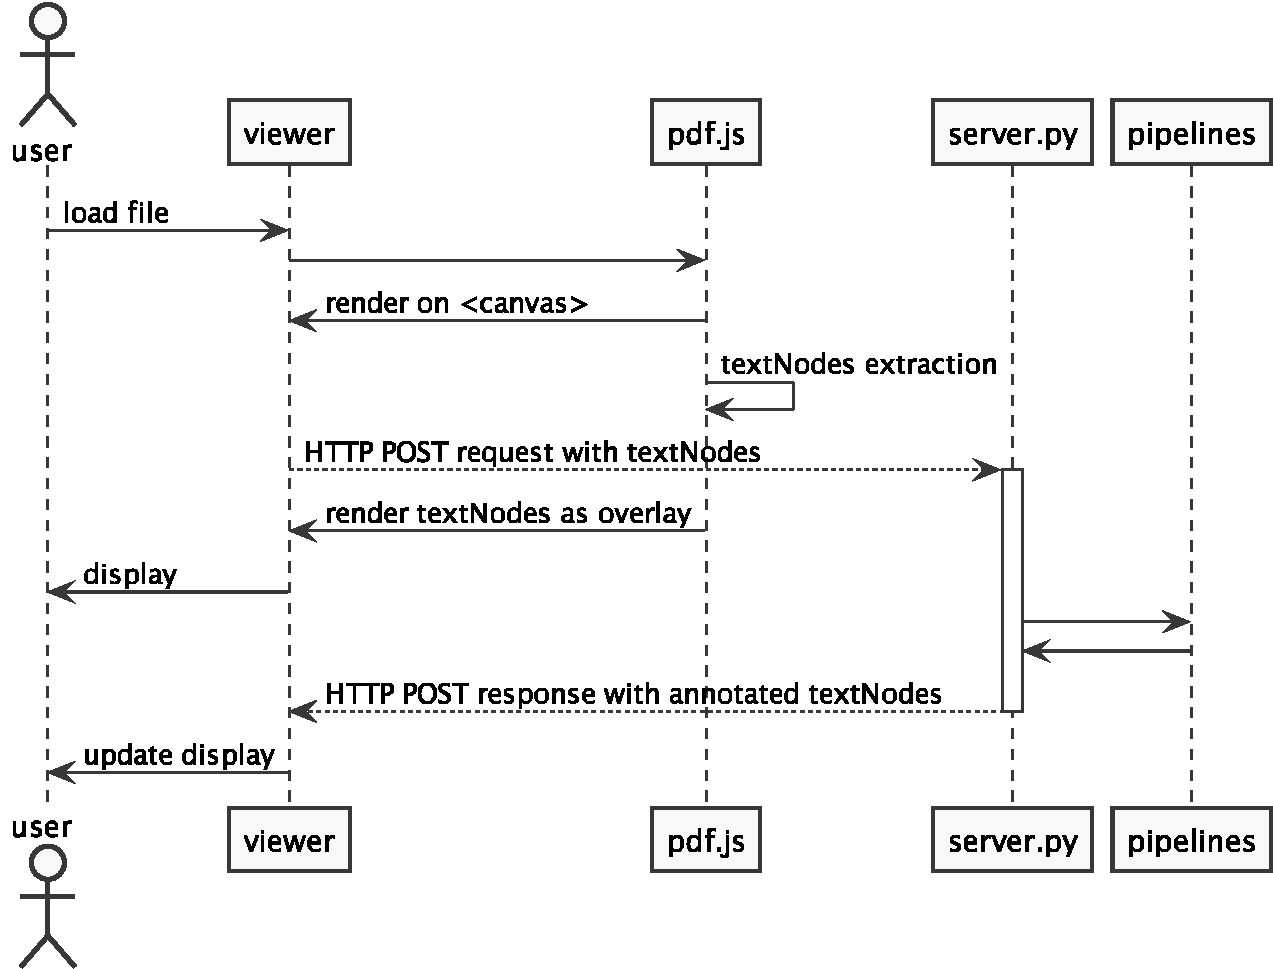
\includegraphics[scale=.275]{./diagrams/sequence.pdf}
\end{center}
\caption{\label{fig:sequence}Sequence diagram of a typical request-response in Spá.}
\vspace{-2em}
\end{wrapfigure}

Spá relies on Mozilla pdf.js\footnote{\url{http://mozilla.github.io/pdf.js}} for visualization of the document and text extraction.
The results of the text extraction are processed server-side by a variety of processing topologies, as outlined in figure \ref{fig:sequence}.
Results, which could come from complicated machine learning systems, are communicated back to the browser and displayed using React components\footnote{\url{http://facebook.github.io/react}}.

For each of the annotations the relevant nodes in the document are highlighted and a custom scrollbar, inspired by \href{http://substance.io/}{substance.io}\footnote{\url{http://substance.io/beta/}}, that acts as a mini-map is projected to show where it resides within the document.
The user can interactively activate and inspect specific results.
\vspace{-1em}

\section{Future work}
We present a web-based tool for interactive visualization of annotations and meta-data on PDF documents.
This allows users to see the results from machine learning predictions for a specific document.
We have demonstrated the utility of this system within the context of \ac{ebm} by automatically extracting potential risks of bias (and supporting sentences) via state-of-the-art ML methods.

More generally, we believe the tool to be potentially useful for a much wider range of text mining and machine learning applications.
To increase the generality of the tool we are developing a pluggable system for processing topologies, allowing developers to quickly plug in new systems for automated PDF annotation.
Furthermore, work is being done on allowing users to save selected annotations, possibly embedded within the document itself, for sharing and off-line use.
The ultimate vision is to have a extensible system for semi-automated (machine assisted) screening, data extraction and data summarization for EBM, and to allow rapid development of similar systems for other domains.

\subsubsection{Acknowledgments}
Part of this research was funded by the European Union Seventh Framework Programme (FP7/2007-2013) under grant agreement n° 261433. % TODO add seed funds ack (BCW)

\bibliographystyle{splncs}
\bibliography{references}

\end{document}
